\documentclass[a4paper, amsfonts, amssymb, amsmath, reprint, showkeys, nofootinbib, twoside]{revtex4-1}
\usepackage[english]{babel}
\usepackage[utf8]{inputenc}
\usepackage[colorinlistoftodos, color=green!40, prependcaption]{todonotes}
\usepackage[pdftex, pdftitle={Article}, pdfauthor={Author}]{hyperref}
\usepackage{amsthm}
\usepackage{mathtools}
\usepackage{physics}
\usepackage{xcolor}
\usepackage{caption}
\usepackage{hyperref}
%\hypersetup{colorlinks=true, linkcolor=blue, urlcolor = blue}
\usepackage{amsmath}
\usepackage{amssymb}
\usepackage{graphicx}
\graphicspath{Images}
\usepackage[left=23mm,right=13mm,top=35mm,columnsep=15pt]{geometry} 
\usepackage{adjustbox}
\usepackage{placeins}
\usepackage[T1]{fontenc}
\usepackage{float}
%\usepackage{longtable}
\usepackage{csquotes}
\usepackage{refstyle}
\usepackage{lipsum}
\usepackage{booktabs}

\begin{document}

\title{Diffraction of light due to ultrasonic wave propagation in liquids}
\author{Swaroop Ramakant Avarsekar}
\email{swaroop.avarsekar@niser.ac.in}
\affiliation{School of Physical Sciences, National Institute of Science Education and Research, HBNI, Jatni -752050, India}
\date{\today}
	
\maketitle

\section{Introduction and Theory}
Ultrasonic waves can be used to create spacing between high and low density regions in the liquid causing similar patterns to that of diffraction grating with some specific frequency. These regions are formed due to compression and rarefaction in the liquid, varying the refractive index. The successive separations between compression and rarefaction is the the wavelength of the oscillation ($\lambda_u$) which is analogous to  grating constant (d) in grating equation.
 
The grating equation changes to 
\begin{equation}
	d.sin\theta=n\lambda\rightarrow\lambda_u.sin\theta=n\lambda
\end{equation}

The velocity of ultrasonic wave in liquid is given by the following equation if we know the wavelength and frequency of oscillation ($\nu$).

\begin{equation}
	V_u=\nu.\lambda_u
\end{equation}

If the velocity of the ultrasound is known then we can calculate the the compressibilty of the liquid (K) and bulk modulus of elasticity (E) with density ($\rho$).

 \begin{equation}
 	V_u=\sqrt{\frac{E}{\rho}}
 \end{equation}
 
 \begin{equation}
 	E=1/K=V_u^2\rho
 \end{equation}
 
The phenomenon of interaction between light and sound waves in a liquid is called Debye-Sears effect.
This method can be used to determine the velocity of sound in liquids, and calculate the compressibilty factor of the same.

\begin{figure}[H] %  figure placement: here, top, bottom, or page
	\centering
	\includegraphics[width=8.3cm,height=5cm]{0} 
	\caption{Diffraction of light due to ultrasonic wave propagation in liquids.\newline \footnotesize{Credit- Shubhang Sharma, SPS, NISER}}
	\label{0}
\end{figure}

\section{Experiment}
\subsection{Apparatus}
We need a radio frequency generator and quartz crystal slab fitted with two leads. Spectrometer is used to calculate the angle of lines. A glass cell to fill the turpentine. The sodium lamp is used as light source.  
\subsection{Procedure}
Sodium lamp is turned on and waited till the light is stabilized. Fill the glass cell with turpentine and place it on the spectrometer. Place the transducer above the cell and lock it in the spectrometer. Connect the leads of  transducer to the radio frequency generator. Setup the radio frequency such that sharp sodium lines are visible in the direction parallel to the source. Measure the angles for up to second order diffraction lines and calculate the required parameters. 

\subsection{Precautions}
\begin{enumerate}
\item{Do not disturb the setup once you start the experiment.}
\item{Tune the frequency very slowly and carefully for sharp and crisp lines.}
\item{Move the screw only in one direction to avoid backlash error.}
\item {Place the crystal parallel to side of cell walls to obtain good standing wave pattern.}

\end{enumerate}

\begin{figure}[H] %  figure placement: here, top, bottom, or page
	\centering
	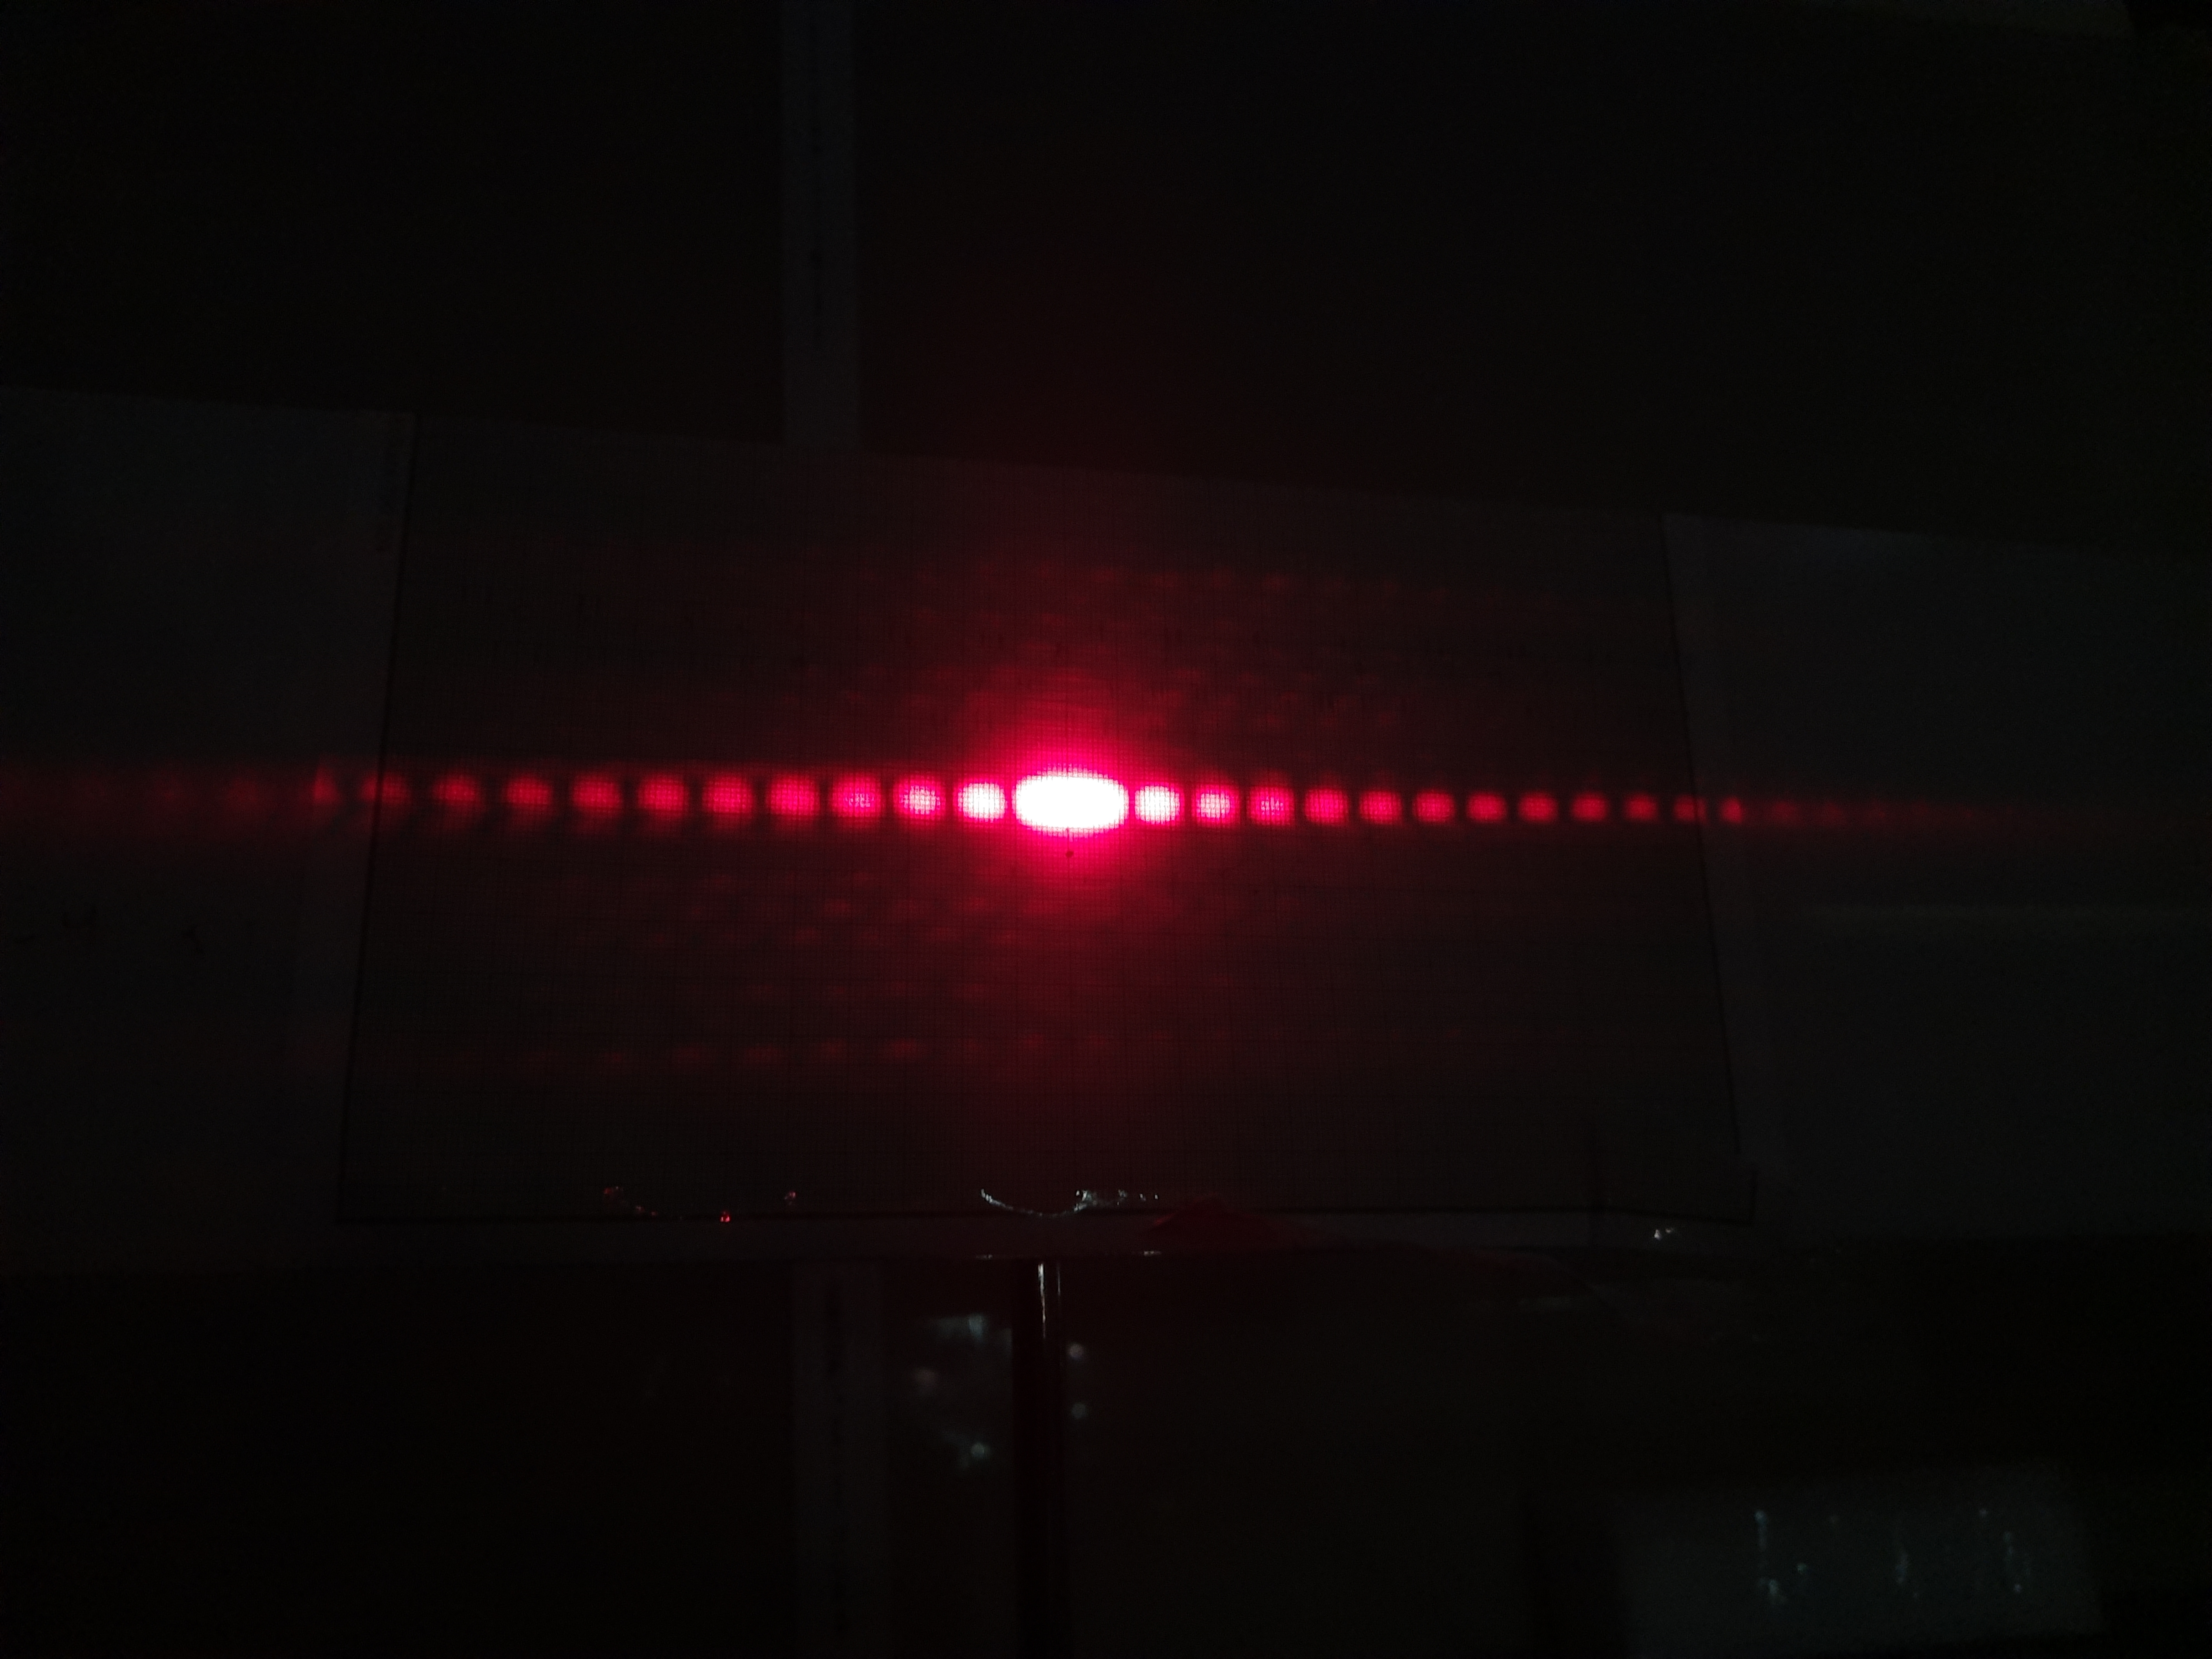
\includegraphics[width=8.3cm, height=5cm]{2} 
	\caption{Experimental setup in Laboratory}
	\label{1}
\end{figure}

\subsection{Observations}
\begin{figure}[H] %  figure placement: here, top, bottom, or page
	\centering
	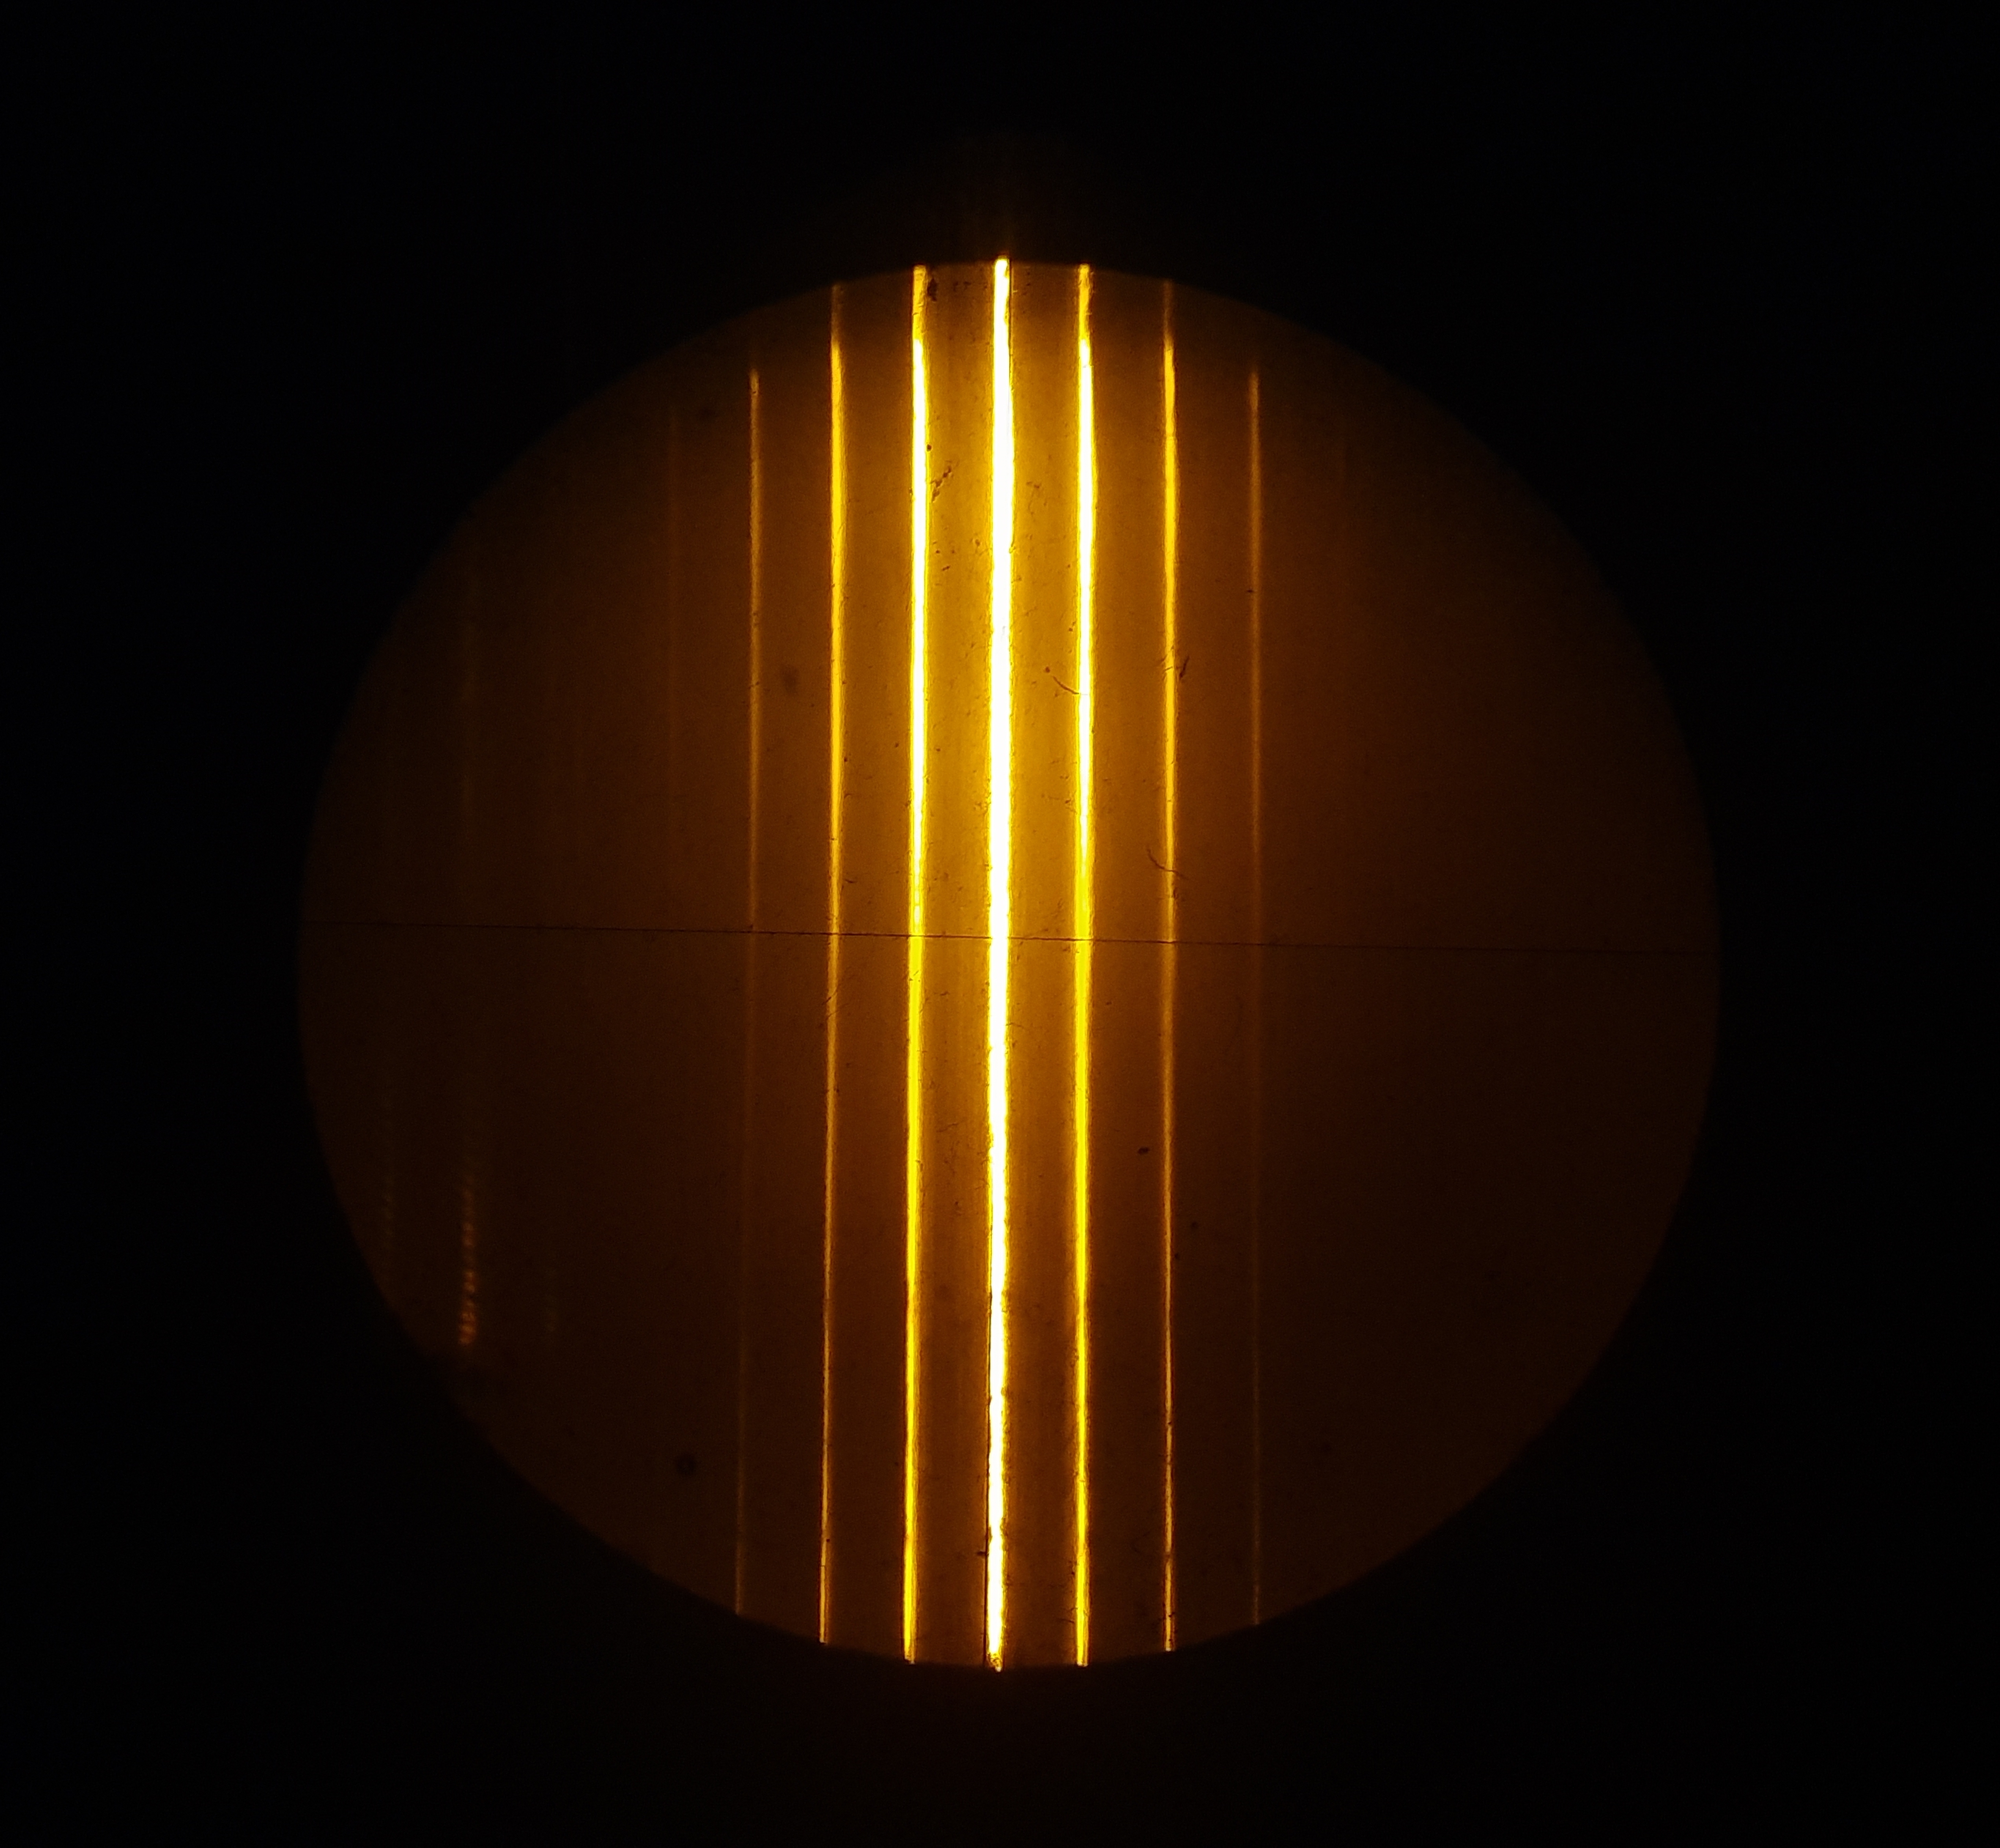
\includegraphics[width=8.3cm,height=6cm]{1} 
	\caption{Sodium diffraction lines visible through spectrometer.}
	\label{2}
\end{figure}


\section{Conclusion}
From the ultrasonic waves through turpentine we were able to setup the diffraction grating in the cell, leading to diffraction lines upto two orders as observed through spectrometer. We found the wavelength of the ultrasound for the first order diffraction pattern to be $(305.40\pm 32.10)\mu m$ and for second order diffraction pattern to be $(299.97\pm 63.41)\mu m$. The average speed of ultrasound in $(1197.56\pm 71.07) m/s$. The bulk modulus and compressibilty of turpentine was found to be $(1.20\pm 0.14)\times10^9 kg m^{-1} s^{-2}$ and $(8.33\pm 0.99)\times10^{-10} ms^{2}kg^{-1}$ respectively. 

The literature value of velocity of ultrasound in turpentine is 1240 m/s at room temperature. The calculated value lies within the range of error bar as compared to literature value with relative error $3.42 \%$. It should also be noted that the velocity of sound is calculated at room temperature ($25^{\circ} C$). The bulk modulus of turpentine is also within the range of literature value of the same i.e $1.28\times10^9$ N m with relative error $6.25 \%$. Several errors like random errors and human errors have contributed to the experiment. The values and error could be minimized by using spectrometer of least count in seconds. With increase in set of readings the value can be improved but due to time constraints it was unable to do so. From the comparison with literature values, this experiment was successful in determining the velocity, bulk modulus and compressibilty of turpentine.  

\section{References}
\begin{enumerate}
\item{\url{https://www.niser.ac.in/sps/sites/default/files/basic_page/Diffraction%20of%20light%20by%20ultrasonic%20waves.pdf}}
\item {\url{https://eng.libretexts.org/Bookshelves/Civil_Engineering/Book%3A_Fluid_Mechanics_(Bar-Meir)/00%3A_Introduction/1.6%3A_Fluid_Properties/1.6.2%3A_Bulk_Modulus}}
\item {\url{https://www.engineeringtoolbox.com/sound-speed-liquids-d_715.html}}
\end{enumerate}
\end{document}